\input{../common/head.tex}
\def\passYear{2016}
\def\faculty{физико-технический институт}
\def\department{Кафедра информационной безопасности}
\def\departmentHead{Н. В. Грайворонский}
\def\kind{Дипломна робота}
\def\level{магістр}
\def\specialityCode{8.04030101}
\def\specialityTitle{Прикладная математика}
\def\theme{Структуры для работы с большими объёмами данных в Python}
\def\gender{female}
\def\mentorGender{male}
\def\course{2}
\def\group{ФИ-41}
\def\name{Лавягина Ольга Алексеевна}
\def\mentorRank{}
\def\mentorName{Колотий Андрей Всеволодович}
\def\reviewerRank{Rank}
\def\reviewerName{Name}
\def\subject{Специальные разделы программирования}


\usepackage{csvsimple}
\usepackage{rotating}
\usepackage{listings}

\begin{document}

\import{1_title/}{title.tex}

\clearpage
\setcounter{page}{2}

%\pagestyle{empty}
\tableofcontents
\thispagestyle{empty}

\clearpage
\pagestyle{fancy}

\clearpage

\chapter{Задание}
В лабораторном задании необходимо:
\begin{enumerate}
\item выполнить параллелизацию известного алгоритма средствами OpenMP. Для этого сначала необходимо реализовать этот алгоритм в последовательном (не параллельном) виде, а потом добавить директивы OpenMP, которые позволяют программе выполнятся параллельно;
\item построить зависимость общего времени выполнения вычислений в программе в зависимости от количества потоков, которое контролируется переменной окружения OMP\_NUM\_THREADS. Максимальное количество потоков, которые используются для построения зависимости, может быть разным, но не меньшим, чем $MIN\left(8, 4\cdot N\right)$, где N --- общее количество вычислительных ядер в системе. Для того, чтобы уменьшить влияние побочных факторов на измерение времени выполнения программы, в качестве тестовых данных следует использовать векторы достаточно большого размера. Время, которое измеряется, не должно включать в себя время, которое тратится на генерацию этих векторов; 
\item исследовать зависимость времени выполнения от использования разных стратегий распределения итераций среди рабочих потоков. Необходимо исследовать стратегии STATIC, DYNAMIC и GUIDED с разными значениями параметра количества итераций. Значение параметра количества итераций следует брать из следующих рядов: \{1, 2, 4, 6, 16, 32, 64\} и \{10\% от M, 10\% от M, ..., 100\% от M\}, где M --- общее количество итераций на поток, которое определяется как полное количество итераций цикла делённое на значени OMP\_NUM\_THREADS.
\end{enumerate}

Порядок выполнения работы:
\begin{enumerate}
\item проанализировать условие задачи;
\item реализовать программу согласно с заданием;
\item построить зависимость времени выполнения программы от количества рабочих потоков;
\item измерить время выполнения программы для разных стратегий распределения итераций в параллельном цикле. Объяснить результаты;
\item результаты работы оформить протоколом. Зависимость времени выполнения от количества потоков и стратегийраспределения итераций следует представить в графическом виде (график и столбиковая диаграмма, соответственно).
\end{enumerate}


Задание: необходимо провести параллелизацию алгоритма из индивидуального задания.


Вариант индивидуального задания: 


1. скалярное произведение векторов, которые состоят из элементов типа double.

\chapter{Листинг кода}
Файл main.h
\lstset{inputencoding=utf8, extendedchars=\true}
\lstinputlisting[language=C,
                 basicstyle=\ttfamily\scriptsize]{source/main.h}

Файл main.c
\lstset{inputencoding=utf8, extendedchars=\true}
\lstinputlisting[language=C,
                 basicstyle=\ttfamily\scriptsize]{source/main.c}
\chapter{Зависимость времени вычисления от количества потоков}

Для построения зависимости времени вычислений от количества потоков, которые контролируются переменной окружения OMP\_NUM\_THREADS (\ref{fig:parallel}), было найдено время для количества потоков от одного до восьми. Максимальное количество потоков, которые используются для постороения зависимости равно $MIN\left(8, 4\cdot N\right)$, где N --- общее количество вычислительный ядер в системе (равно двум).

Для того, чтобы уменьшить влияние побочных факторов на измерение времени выполнения программы, в качестве тестовых данных были использованы векторы с размером $10^8$. Время, которое измеряется, включает в себя только время, которое тратится на вычисление скалярного произведения векторов.

\begin{table}[h]
  \centering
  \csvreader[tabular=|l|c|,
  table head=\hline Количество потоков & Время \\\hline,
  late after line=\\\hline]
  {source/parallel.csv}{numberofthreads=\threads,time=\time}
  {\threads & \time}

  \caption{Время выполнения вычислений для разного количества потоков}
  \label{tab:parallel}
\end{table}

\begin{figure}[h]
  \centering
  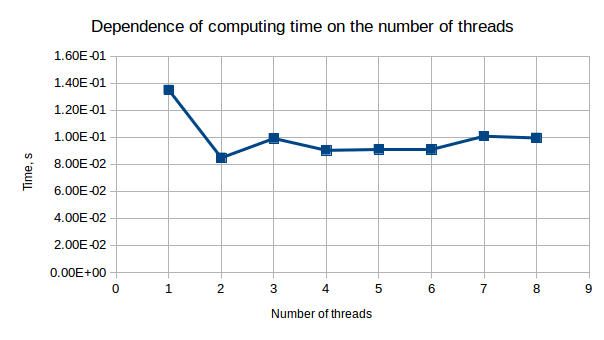
\includegraphics[width=.75\textwidth]{parallel.png}
  \caption{Зависимость времени вычисления от количества потоков}
\label{fig:parallel}
\end{figure}

\chapter{Стратегия STATIC}

\lstset{language=C}
\begin{lstlisting}
schedule(static, block_size)
\end{lstlisting}

В данной стратегии все шаги цикла делятся на блоки указанного размера. Каждой задаче назначается приблизительно равное количество блоков. Один блок назначается одной задаче. Таким образом, планировщик static назначает приблизительно равное количество шагов цикла каждой задаче.

Значение параметра количества итераций бралось из ряда {1, 2, 4, 8, 16, 32, 64} (\ref{fig:static}).

\begin{sidewaystable}[h]
  \centering
  \csvreader[tabular=|l|l|l|l|l|l|l|l|,
  table head=\hline Количество итераций & 2 потока & 3 потока & 4 потока & 5 потоков & 6 потоков & 7 потоков & 8 потоков \\\hline,
  late after line=\\\hline]
  {source/static.csv}{iterations=\iterations,two=\two,three=\three,four=\four,five=\five,six=\six,seven=\seven,eight=\eight}
  {\iterations & \two & \three & \four & \five & \six & \seven & \eight}

  \caption{Время выполнения вычислений для разного количества потоков для разного количества итераций при стратегии STATIC}
  \label{tab:static}
\end{sidewaystable}

\begin{figure}[h]
  \centering
  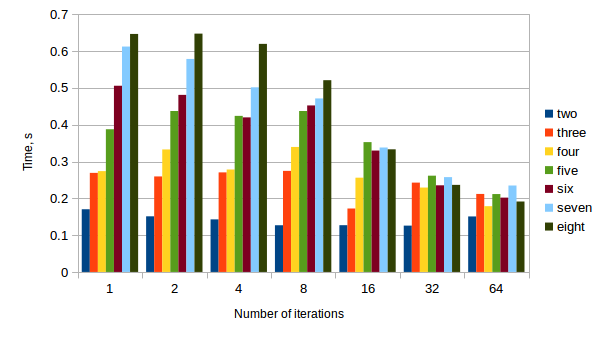
\includegraphics[width=.75\textwidth]{static.png}
  \caption{Зависимость времени вычисления от количества итераций при разном количестве потоков для стратегии STATIC}
\label{fig:static}
\end{figure}

В следующей зависимости (\ref{fig:staticm}) параметр количества итераций брался из ряда \{10\% от M, 10\% от M, ..., 100\% от M\}, где M --- общее количество итераций на поток, которое определяется как полное количество итераций цикла (размер вектора, то есть $10^8$) делённое на значение OMP\_NUM\_THREADS (8), следовательно $M = \frac{10^8}{8} = 12500000$.

\begin{table}[h]
  \centering
  \csvreader[tabular=|l|c|,
  table head=\hline Количество итераций & Время \\\hline,
  late after line=\\\hline]
  {source/static_m.csv}{iterations=\iterations,time=\time}
  {\iterations & \time}

  \caption{Время выполнения вычислений для восьми потоков для разного количества итераций для стратегии STATIC}
  \label{tab:staticm}
\end{table}

\begin{figure}[h]
  \centering
  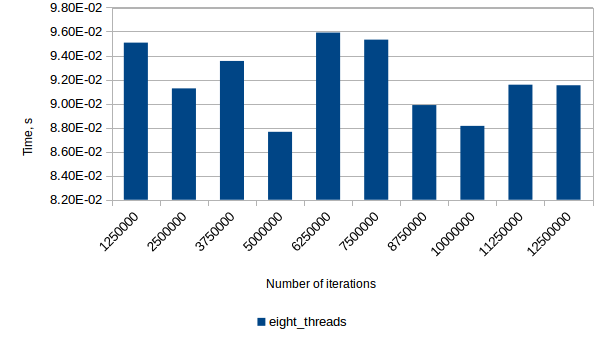
\includegraphics[width=.75\textwidth]{static_m.png}
  \caption{Зависимость времени вычисления от количества итераций при восьми потоках для стратегии STATIC}
\label{fig:staticm}
\end{figure}

\chapter{Стратегия DYNAMIC}

\lstset{language=C}
\begin{lstlisting}
schedule(dynamic, block_size)
\end{lstlisting}

Все шаги цикла делятся на блоки указанного размера. Каждой задаче назначается по одному блоку. Когда задача закончила выполнение блока, ей назначается ещё не назначенный блок, и так до того, пока ещё есть не назначенные блоки.

Таким образом, планировщик dynamic назначает шаги цикла задачам так, чтобы задачи выполняли директиву for приблизительно равное время.

Значение параметра количества итераций бралось из ряда {1, 2, 4, 8, 16, 32, 64} (\ref{fig:dynamic}).

\begin{sidewaystable}[h]
  \centering
  \csvreader[tabular=|l|l|l|l|l|l|l|l|,
  table head=\hline Количество итераций & 2 потока & 3 потока & 4 потока & 5 потоков & 6 потоков & 7 потоков & 8 потоков \\\hline,
  late after line=\\\hline]
  {source/dynamic.csv}{iterations=\iterations,two=\two,three=\three,four=\four,five=\five,six=\six,seven=\seven,eight=\eight}
  {\iterations & \two & \three & \four & \five & \six & \seven & \eight}

  \caption{Время выполнения вычислений для разного количества потоков для разного количества итераций при стратегии DYNAMIC}
  \label{tab:dynamic}
\end{sidewaystable}

\begin{figure}[h]
  \centering
  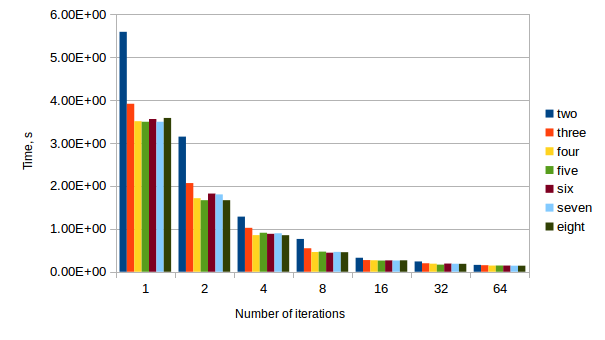
\includegraphics[width=.75\textwidth]{dynamic.png}
  \caption{Зависимость времени вычисления от количества итераций при разном количестве потоков для стратегии DYNAMIC}
\label{fig:dynamic}
\end{figure}

В следующей зависимости (\ref{fig:dynamicm}) параметр количества итераций брался из ряда \{10\% от M, 10\% от M, ..., 100\% от M\}, где M --- общее количество итераций на поток, которое определяется как полное количество итераций цикла (размер вектора, то есть $10^8$) делённое на значение OMP\_NUM\_THREADS (8), следовательно $M = \frac{10^8}{8} = 12500000$.

\begin{table}[h]
  \centering
  \csvreader[tabular=|l|c|,
  table head=\hline Количество итераций & Время \\\hline,
  late after line=\\\hline]
  {source/dynamic_m.csv}{iterations=\iterations,time=\time}
  {\iterations & \time}

  \caption{Время выполнения вычислений для восьми потоков для разного количества итераций для стратегии DYNAMIC}
  \label{tab:dynamicm}
\end{table}

\begin{figure}[h]
  \centering
  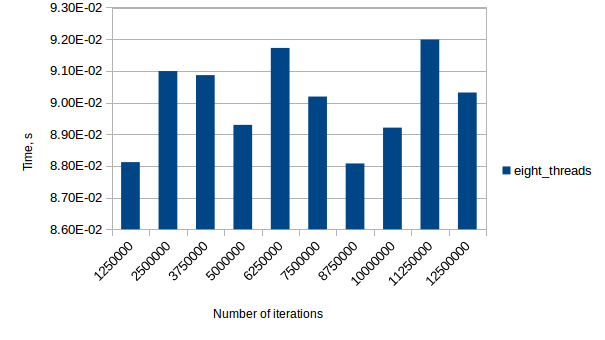
\includegraphics[width=.75\textwidth]{dynamic_m.png}
  \caption{Зависимость времени вычисления от количества итераций при восьми потоках для стратегии DYNAMIC}
\label{fig:dynamicm}
\end{figure}

\chapter{Стратегия GUIDED}

\lstset{language=C}
\begin{lstlisting}
schedule(guided, block_size)
\end{lstlisting}

Ещё не выполненные шаги цикла делятся на блоки размером, пропорциональным $\frac{N}{P}$ (N --- количество шагов цикла), но не меньше, чем размер блока. Каждый из сформированных блоков назначается задачам. Когда задача закончила выполнение блока, для неё формируется новый блок по тому же правилу. Таким образом, размеры блоков со временем уменьшаются до указанного block\_size.

Значение параметра количества итераций бралось из ряда {1, 2, 4, 8, 16, 32, 64} (\ref{fig:guided}).

\begin{sidewaystable}[h]
  \centering
  \csvreader[tabular=|l|l|l|l|l|l|l|l|,
  table head=\hline Количество итераций & 2 потока & 3 потока & 4 потока & 5 потоков & 6 потоков & 7 потоков & 8 потоков \\\hline,
  late after line=\\\hline]
  {source/guided.csv}{iterations=\iterations,two=\two,three=\three,four=\four,five=\five,six=\six,seven=\seven,eight=\eight}
  {\iterations & \two & \three & \four & \five & \six & \seven & \eight}

  \caption{Время выполнения вычислений для разного количества потоков для разного количества итераций при стратегии GUIDED}
  \label{tab:guided}
\end{sidewaystable}

\begin{figure}[h]
  \centering
  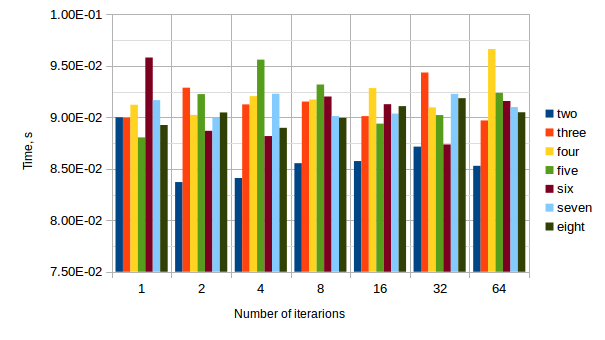
\includegraphics[width=.75\textwidth]{guided.png}
  \caption{Зависимость времени вычисления от количества итераций при разном количестве потоков для стратегии GUIDED}
\label{fig:guided}
\end{figure}

В следующей зависимости (\ref{fig:guidedm}) параметр количества итераций брался из ряда \{10\% от M, 10\% от M, ..., 100\% от M\}, где M --- общее количество итераций на поток, которое определяется как полное количество итераций цикла (размер вектора, то есть $10^8$) делённое на значение OMP\_NUM\_THREADS (8), следовательно $M = \frac{10^8}{8} = 12500000$.

\begin{table}[h]
  \centering
  \csvreader[tabular=|l|c|,
  table head=\hline Количество итераций & Время \\\hline,
  late after line=\\\hline]
  {source/guided_m.csv}{iterations=\iterations,time=\time}
  {\iterations & \time}

  \caption{Время выполнения вычислений для восьми потоков для разного количества итераций для стратегии GUIDED}
  \label{tab:guidedm}
\end{table}

\begin{figure}[h]
  \centering
  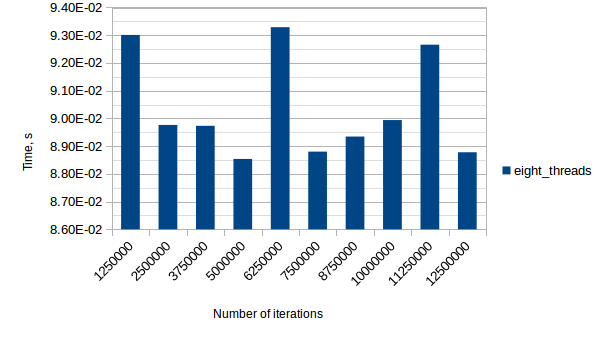
\includegraphics[width=.75\textwidth]{guided_m.png}
  \caption{Зависимость времени вычисления от количества итераций при восьми потоках для стратегии GUIDED}
\label{fig:guidedm}
\end{figure}

\chapter*{Выводы}
\addcontentsline{toc}{chapter}{Выводы}

При исследовании зависимости времени вычисления от количества потоков (\ref{fig:parallel}) было обнаружено, что с увеличением числа потоков время увеличивается. Это можно объяснить тем, что оно тратится на создание потоков.

Лучше всего зависимость времени вычисления от количества итераций прослеживается при использовании стратегии DYNAMIC (\ref{fig:dynamic}). При увеличении количества итераций время вычислений уменишается.


\end{document}
